\chapter{Marco Teórico}

\section{Cuerpo de agua}
Un cuerpo de agua es cualquier extensión que se encuentran en la superficie terrestre (ríos y lagos) o en el subsuelo (acuíferos, ríos subterráneos); tanto en estado líquido, como sólido (glaciares, casquetes polares); tanto naturales como artificiales (embalses) y pueden ser de agua salada o dulce\cite{agua2024}.

La RENAMECA establece que cuerpos de agua pueden clasificarse como lénticos (agua en reposo como lagos y estanques), lóticos (masas de agua en movimiento constante, como ríos y arroyos), costeros (aguas costeras como playas, bahías, marismas y estuarios) y subterráneos (aguas del subsuelo como pozos, cenotes, galerías y manantiales)

%referencia RENAMECA https://app.conagua.gob.mx/ICA/Contenido?n1=1&n2=1 . 
Este proyecto se enfoca principalmente en cuerpos de agua lóticos debido a la necesidad de monitoreo continuo, ya que en ellos suelen realizarse descargas industriales y agrícolas, albergan una vida acuática importante y, en muchas ocasiones, actúan como proveedores de agua para diversos fines. 

\section{Calidad del Agua}
La calidad del agua se refiere a la condición general y a las características físicas, químicas y biológicas que permiten su uso para un determinado fin, ayudaran a determinar si es apta, por ejemplo, para consumo humano, riego agrícola, protección de la vida acuática o uso recreativo. 
La evaluación de la calidad del agua requiere el monitoreo de parámetros clave como pH, oxígeno disuelto, turbidez, temperatura y conductividad, entre otros parámetros químicos, los cuales proporcionan información crítica sobre el estado del ecosistema acuático y la posible presencia de contaminantes.
La solución propuesta integra una red inalámbrica de sensores (WSN) y un sistema de visión artificial, permitiendo un monitoreo continuo y automatizado que mejora la precisión al evitar errores asociados al transporte y almacenamiento de muestras.

\section{Contaminación}
El término contaminación se refiere a la introducción de cualquier agente químico, físico o biológico cuya presencia o acumulación tiene efectos nocivos en el entorno natural,  la salud y el bienestar de las personas.La magnitud de su impacto generalmente depende de una combinación de aspectos como la cantidad, el tipo de contaminante, la vía de ingreso  y el tipo de medio al que se incorporan.

Se dice que el agua está contaminada cuando los agentes contaminantes repercuten negativamente en su calidad para el consumo humano, para usos posteriores o para el bienestar de los ecosistemas. Es la contaminación que ocurre en cualquier espacio que alberga agua: ríos, lagos, acuíferos o incluso el mar \cite{agua2024contaminacion}. 


\section{Parámetros de la calidad del agua}

\subsection{pH}
El pH del agua afecta procesos como la corrosión y las incrustaciones en redes de distribución. Aunque no tiene un impacto directo en la salud, influye en el tratamiento del agua, especialmente en la coagulación y desinfección. Las aguas naturales suelen tener un pH entre 5 y 9 \cite{uno2020}. 


En México, los niveles recomendados de pH para agua potable están regulados por la NOM-127-SSA1-2021, que establece los límites de calidad del agua para uso y consumo humano. Según esta norma, el pH del agua debe encontrarse dentro de un rango de 6.5 a 8.5 para garantizar su potabilidad y evitar problemas como corrosión o incrustaciones en las redes de distribución \cite{uno2020}.

Este rango busca no solo proteger los equipos de distribución, sino también asegurar la eficiencia en los procesos de tratamiento, como la desinfección, y garantizar que el agua sea apta para el consumo humano \cite{uno2020}.

\subsection{Turbiedad}
La turbidez del agua se produce por partículas en suspensión, como arcillas, limo y tierra fina, que reducen su transparencia. Se mide usando turbidímetros o nefelómetros, en unidades nefelométricas de turbidez (UNT). Para mantener la calidad del agua potable, las normas recomiendan no superar 5 UNT, y para una desinfección eficiente, el agua filtrada debería tener menos de 1 UNT\cite{uno2020}

\subsection{Conductividad}
El agua pura es un mal conductor de la electricidad, pero cuando contiene sales se convierte en un buen conductor porque hay presencia de iones con cargas eléctricas. La conductividad electrolítica es una expresión numérica de la capacidad de una solución para transportar una corriente eléctrica. Esta capacidad depende de la presencia de iones, de su concentración total, de su movilidad, valencia y concentraciones relativas, así como de la temperatura \cite{nmx2000}.

\subsection{Temperatura}
La temperatura es un parámetro físico clave en el agua, ya que afecta procesos biológicos y químicos como la actividad microbiana, la absorción de oxígeno, la precipitación de compuestos y la eficiencia en la desinfección. También influye en operaciones de tratamiento como la mezcla, floculación, sedimentación y filtración. La temperatura del agua varía constantemente debido a factores ambientales \cite{uno2020}.

La integración de sensores en la solución propuesta permite monitorear continuamente la temperatura, ajustando las mediciones de otros parámetros como la conductividad, que depende directamente de este valor. Esto asegura un análisis más preciso y adaptado a las condiciones dinámicas de los cuerpos de agua monitoreados.

\subsection{Oxigeno Disuelto}
El oxígeno disuelto (OD) es fundamental para la supervivencia de los organismos acuáticos, ya que la mayoría de las especies dependen de niveles adecuados de oxígeno en el agua. Factores como la temperatura y la actividad biológica influyen en su concentración. A mayor temperatura, menor capacidad del agua para retener oxígeno. Además, la medición del OD puede proporcionar información valiosa sobre la presencia de contaminantes, como materia orgánica en descomposición o vertidos industriales, que disminuyen los niveles de oxígeno en el agua, afectando negativamente a la vida acuática. Los valores recomendados para cuerpos de agua que soportan vida acuática oscilan entre 5 y 8 mg/L, dependiendo de las condiciones locales \cite{swamp2023}.


%\subsection{Sensor de pH}
%Es un dispositivo que se utiliza para medir la acidez o alcalinidad de una solución, mediante la detección de la concentración de iones de hidrógeno.
Los parámetros básicos, como pH, oxígeno disuelto, turbidez, conductividad y temperatura, son indicadores fundamentales del estado de los cuerpos de agua. Estos permiten identificar la presencia de contaminantes, evaluar la salud de los ecosistemas acuáticos y determinar la aptitud del agua para diferentes usos. Su monitoreo es clave para detectar cambios asociados a actividades humanas, como descargas industriales y agrícolas, y para garantizar la sostenibilidad de los recursos hídricos.

\section{Monitoreo del agua}
Se entiende por el proceso constante de observación, medición y análisis de parámetros que dan indicio de la calidad del agua. El monitoreo del agua permite conocer su calidad a través del tiempo, la cual se determina analíticamente por diferentes parámetros físicos, químicos y biológicos, en función del uso al cual va a ser destinada \cite{monitoreo2023}.


\section{Sensores}
Los sensores son dispositivos hardware que producen una respuesta medible ante un cambio en un estado
físico, como puede ser temperatura o presión. Los sensores detectan o miden cambios físicos en el área
que están monitorizando. La señal analógica continua detectada es digitalizada por un convertidor
analógico digital y enviada a un controlador para ser procesada.
Las características y requerimientos que un sensor debe tener son un pequeño tamaño, un consumo bajo
de energía, operar en densidades volumétricas altas, ser autónomo y funcionar desatendidamente y tener
capacidad para adaptarse al ambiente \cite{fernandez2009}.
Los sensores pueden estar clasificados en tres categorías:
\begin{itemize}
    \item Sensores pasivos omnidireccionales: Los sensores pasivos captan los datos sin necesidad de
manipular el entorno. Son autoalimentados y solo usan la energía para amplificar la señal
analógica captada. No hay ninguna noción de 'dirección' involucrada en estas mediciones.
    \item Sensores pasivos unidireccionales: Son sensores pasivos que tienen bien definida la dirección
desde donde deben captar la información. Un ejemplo típico es una cámara.
    \item Sensores activos: Este tipo de sensores sondean el ambiente, por ejemplo un radar, o algún tipo de sensor sísmico que generan ondas expansivas a través de pequeñas explosiones.
\end{itemize}


\section{Sensores para medir la calidad del agua}
 \begin{itemize}
    
        \item \textbf{Sensores de pH:} Detectan variaciones en la acidez del agua, asociadas a posibles vertidos industriales o agrícolas que alteran el equilibrio químico del ecosistema. Los sensores de pH suelen utilizar un electrodo de vidrio que mide la actividad de los iones de hidrógeno en el agua. El sensor produce un voltaje proporcional al nivel de pH, que luego se muestra en un medidor \cite{waterQualitySensors}.
        
        \item \textbf{Sensores de Turbidez:} Miden la claridad del agua para identificar la presencia de residuos sólidos en suspensión, lo que podría estar relacionado con actividades de minería o construcción cercanas.
        Los sensores de turbidez funcionan haciendo brillar una luz a través del agua y midiendo la cantidad de luz dispersada por las partículas. Cuanto mayor es la turbidez, más luz se dispersa \cite{waterQualitySensors}.
        
        \item \textbf{Sensores de Temperatura:} Detectan cambios abruptos en la temperatura, los cuales podrían señalar descargas de aguas industriales o vertidos térmicos que afectan la fauna acuática. Además, la medición precisa de la temperatura es fundamental para mejorar las lecturas del sensor de conductividad, ya que la conductividad del agua varía con la temperatura. Integrar ambas lecturas permite ajustar los valores de conductividad en función de las fluctuaciones térmicas.
        Los sensores de temperatura suelen utilizar termistores o detectores de temperatura de resistencia (RTD) que cambian la resistencia con la temperatura. El cambio de resistencia se convierte en una lectura de temperatura \cite{waterQualitySensors}.
        
        \item \textbf{Sensores de Oxigenación:} Miden el nivel de oxígeno disuelto en el agua, un parámetro crítico para la vida acuática. La disminución de oxígeno puede ser un indicio de contaminación orgánica o inorgánica que afecte la salud del ecosistema. 
        Estos sensores suelen utilizar métodos electroquímicos u ópticos. En los sensores electroquímicos, el oxígeno se difunde a través de una membrana y reacciona en un electrodo, generando una corriente proporcional a la concentración de oxígeno. Los sensores ópticos miden la extinción de un tinte luminiscente por el oxígeno \cite{waterQualitySensors}.

        \item \textbf{Sensores de Conductividad:} Miden la capacidad del agua para conducir corriente eléctrica, lo cual está relacionado directamente con la cantidad de iones disueltos (sales, minerales y otros compuestos) presentes en el agua. 
        Los sensores de conductividad utilizan electrodos para hacer pasar una pequeña corriente eléctrica a través del agua. La conductividad se determina midiendo la caída de voltaje a través de los electrodos \cite{waterQualitySensors}.
        %referencias: https://sensor1stop.com/es/knowledge/water-quality-sensors/ es la misma para todos los parametros, poner al final de cada parrafo
        
    \end{itemize}

Los sensores representan una solución innovadora para medir parámetros de calidad del agua de forma continua y precisa. A diferencia de los métodos manuales, estos dispositivos permiten la recolección de datos en tiempo real, incluso en condiciones ambientales adversas. Al integrarse en redes inalámbricas, los sensores facilitan la transmisión inmediata de datos a sistemas de procesamiento, lo que optimiza su análisis y visualización
    
\section{Red inalámbrica de Sensores}

Las redes inalámbricas de sensores (WSN, por sus siglas en inglés) están conformadas por un conjunto de nodos sensores autónomos que se comunican entre sí de manera inalámbrica para monitorear variables del entorno y transmitir los datos recolectados hacia un nodo central o estación base. Estos sistemas son ampliamente utilizados en aplicaciones como monitoreo ambiental, control de infraestructuras, agricultura inteligente, seguridad, entre otros.

Uno de los estándares más utilizados en estas redes es el IEEE 802.15.4, el cual define especificaciones para la capa física y la capa de enlace. Sobre estas capas operan diversos protocolos, como Zigbee, WirelessHART, ISA100.11a y 6LowPAN, que permiten establecer la comunicación entre nodos sensores de manera eficiente y escalable.

En contextos de monitoreo de infraestructuras lineales a gran escala —como ríos, oleoductos o fronteras— se emplea un tipo particular de WSN con topología lineal. Estas redes se caracterizan por disponer los nodos a lo largo de una línea o trayectoria determinada, donde cada nodo actúa como retransmisor hacia el siguiente, formando una cadena de comunicación hasta llegar al nodo colector. Dado que la mayoría de los nodos se encuentra fuera del rango directo del nodo frontera, la comunicación se realiza mediante múltiples saltos (\textit{multi-hop}) \cite{egas2021red}.

\begin{figure}[H]
    \centering
    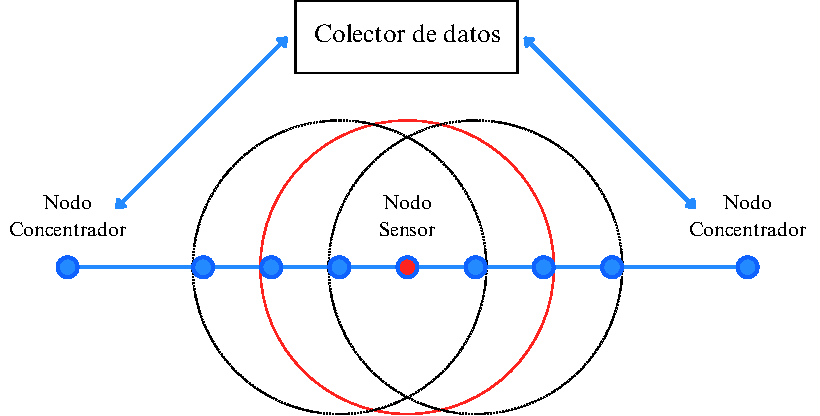
\includegraphics[width=0.8\linewidth]{Documento/Imagenes/Marco Teorico/Topologia lineal.pdf}
    \caption{Topología Lineal}
    \label{fig:topologia_lineal}
\end{figure}


\subsection{Características de las Redes con Topología Lineal}

Las redes inalámbricas de sensores con topología lineal presentan desafíos y ventajas específicas:

\begin{itemize}
    \item \textbf{Bajo consumo energético:} Los nodos operan con baterías, por lo que los protocolos deben minimizar el procesamiento y las retransmisiones innecesarias para extender la vida útil de la red.
    \item \textbf{Infraestructura fija y predictable:} La ubicación secuencial y estática de los nodos permite asignar identificadores automáticamente sin necesidad de protocolos complejos de direccionamiento.
    \item \textbf{Rutas definidas por defecto:} Al existir una única trayectoria de comunicación hacia el nodo frontera, no es necesario implementar capas de red completas ni algoritmos de enrutamiento convencionales.
    \item \textbf{Escalabilidad:} Estas redes pueden extenderse fácilmente a lo largo de grandes distancias sin necesidad de rediseñar la topología.
    \item \textbf{Limitaciones de cómputo:} Dado que los nodos son de bajo costo y con recursos limitados, se recomienda eliminar funciones innecesarias, como la capa de red, para reducir complejidad y consumo.
\end{itemize}

\begin{comment}
\subsection*{Ventajas para Monitoreo Ambiental}

Este tipo de redes es especialmente adecuado para el monitoreo de cuerpos de agua como ríos, ya que:

\begin{itemize}
    \item Permiten cubrir grandes tramos longitudinales con una cantidad razonable de nodos.
    \item Pueden operar durante largos periodos sin intervención humana gracias a su bajo consumo energético.
    \item Su arquitectura simplificada reduce los costos de implementación y mantenimiento.
\end{itemize}

Por estas razones, las WSN con topología lineal representan una solución viable y eficiente para proyectos de monitoreo ambiental distribuido, como el que se propone en este trabajo.
\end{comment}



\begin{comment}
    

\subsection{Nodos}
Las WSN o redes inalámbricas de sensores están compuestas por nodos de bajo costo y bajo consumo de energía que pueden recolectar información del medio ambiente, procesarla y enviarla a través de conexiones inalámbricas a un nodo central de coordinación. Los nodos actúan como parte de la 
infraestructura de comunicaciones, retransmitiendo los mensajes de los nodos más alejados hasta llegar al centro de coordinación.  La red de sensores inalámbricos está formada por numerosos dispositivos distribuidos espacialmente, que utilizan sensores para monitorear diversas condiciones en distintos puntos, entre ellas la temperatura, el sonido, la vibración, la presión y movimiento o los contaminan
tes. Los sensores pueden ser fijos o móviles\cite{fernandez2008}. Los dispositivos son unidades autónomas que constan de un microcontrolador, una fuente de energía (casi siempre una batería), un
 radio transceptor(RF), un elemento sensor y en de manera opcional actuadores. 

En la figura [\ref{fig:Componentes_nodo}] se muestran los componentes que conforman a un nodo\cite{fernandez2009}.
\begin{figure}[H]
    \centering
    %\includegraphics[width=0.5\linewidth]{nodos.png}
    \includegraphics[width=0.6\linewidth]{Documento/Imagenes/compNodoSen.png}
    %\caption{Componentes que conforman a un nodo \cite{fernandez2008}}
    \caption{Componentes que conforman a un nodo}
    \label{fig:Componentes_nodo}
\end{figure}

\begin{enumerate}
    \item \textbf{Procesador:} 
    Es el componente que interpreta y procesa los datos para transmitirlos a otra estación. También gestiona el almacenamiento de datos en la memoria. Puesto que de un nodo sensor se espera una comunicación y una recogida de datos mediante sensores, debe existir una unidad de procesado que se encargue de gestionar todas estas operaciones \cite{fernandez2009}.
    \item \textbf{Sensor:} 
    Los sensores son dispositivos hardware que producen una respuesta medible ante un cambio en un estado físico, como puede ser temperatura o presión. Los sensores detectan o miden cambios físicos en el área que están monitoreando. La señal analógica continua detectada es digitalizada por un convertidor analógico-digital y enviada a un controlador para ser procesada. Las características y requerimientos que un sensor debe tener son un pequeño tamaño, un consumo bajo de energía, operar en densidades volumétricas altas, ser autónomo y funcionar desatendidamente, además de tener capacidad para adaptarse al ambiente \cite{fernandez2009}.

    \item \textbf{Transceptor:} 
    El dispositivo de comunicación utilizado por los nodos en una WSN es un dispositivo vía radio que se comunica con otros dispositivos dentro de su rango de transmisión. Los nodos utilizan la banda ISM, que es una banda reservada para uso no comercial de radiofrecuencia electromagnética en áreas industriales, científicas y médicas. Esta banda de frecuencia está disponible para todo el mundo sin necesidad de licencia, siempre que se respeten las regulaciones que limitan los niveles de potencia transmitida \cite{fernandez2009}. Los medios a elegir para realizar una comunicación inalámbrica son varios: radiofrecuencia, comunicación óptica mediante láser e infrarrojos. La radiofrecuencia (RF) es la más adecuada para usar en aplicaciones inalámbricas. Las WSN usan las frecuencias de comunicación que van entre 433 MHz y 2.4 GHz. El transceptor es un dispositivo que combina las funciones de emisión y recepción. Tiene diferentes estados de operación, incluyendo el modo de emisión, el modo de recepción, el modo de dormir y el modo de inactividad. En los modelos actuales de transceptor, el modo de inactividad consume casi la misma cantidad de energía que el modo de recepción, por lo que es mejor apagar completamente las comunicaciones de radio cuando no se están emitiendo ni recibiendo. Además, el cambio de modo de dormir a transmisión de datos también consume una cantidad significativa de energía \cite{fernandez2009}.
\end{enumerate}
\end{comment}
\subsection{Tipos de nodos en una WSN}

Los nodos son los elementos fundamentales de una red inalámbrica de sensores (WSN), y están diseñados para operar de manera autónoma en entornos distribuidos. Cada nodo es capaz de sensar parámetros físicos, realizar un procesamiento básico local y transmitir la información recolectada hacia otros nodos o un nodo recolector (sink), a través de enlaces inalámbricos.
\subsubsection*{Nodo Sensor}
La arquitectura típica de un nodo sensor está compuesta por cuatro módulos principales:

\begin{itemize}
    \item \textbf{Módulo de sensado:} Incluye sensores encargados de capturar variables del entorno, como temperatura, humedad, presión, vibraciones, entre otros. Los datos analógicos son digitalizados mediante un convertidor ADC (Analógico-Digital) para su posterior procesamiento.
    
    \item \textbf{Unidad de procesamiento:} Se encarga de controlar el nodo, ejecutar rutinas de sensado, realizar tareas básicas de filtrado o compresión de datos, y gestionar las operaciones de transmisión.
    
    \item \textbf{Módulo de comunicación inalámbrica:} Utiliza tecnologías como Zigbee, 6LowPAN o protocolos basados en IEEE 802.15.4. Este módulo permite enviar y recibir datos entre nodos en configuraciones ad hoc de múltiples saltos.
    
    \item \textbf{Fuente de energía:} Usualmente se emplean baterías de larga duración. Dado que el reemplazo o recarga puede no ser viable, la eficiencia energética es un factor crítico. Algunas aplicaciones avanzadas incorporan sistemas de recolección de energía ambiental (harvesting).
\end{itemize}

Dependiendo de la aplicación, los nodos pueden estar complementados con otros elementos como sistemas de localización o actuadores. Además, pueden desplegarse de forma fija o móvil, en espacios abiertos, ambientes industriales o entornos hostiles.

En el contexto de aplicaciones como el monitoreo ambiental de ríos, los nodos se despliegan linealmente a lo largo del cauce, formando una red multisalto donde cada nodo transmite sus datos y actúa como repetidor de otros. Esta función requiere una arquitectura eficiente, ya que cada retransmisión incrementa el consumo energético y los retardos de comunicación.

Dado que los nodos operan frecuentemente en condiciones de aislamiento, deben ser tolerantes a fallos. Esto implica que la red debe seguir funcionando aun si algunos nodos fallan por pérdida de energía, daño físico o interferencias ambientales. Por esta razón, los protocolos utilizados deben ser robustos, autoorganizados y adaptables al entorno \cite{perez2014metodologia}.

El diseño del nodo y la elección de sus componentes deben considerar: tamaño, autonomía, capacidad de cómputo, tipo de sensor, alcance de transmisión, y compatibilidad con la topología de red definida (estrella, malla, lineal, etc.). Estas decisiones impactan directamente en la escalabilidad, fiabilidad y costo del sistema completo.

\begin{figure}[H]
    \centering
    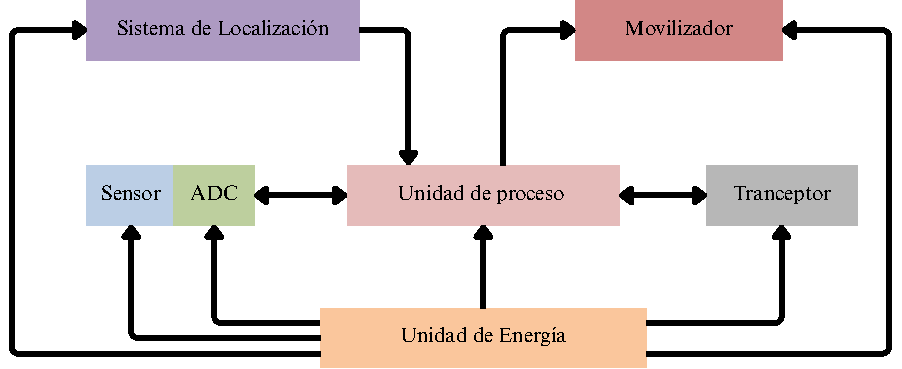
\includegraphics[width=0.6\linewidth]{Documento/Imagenes/Marco Teorico/Nodo sensor.pdf}
    \caption{Componentes que conforman a un nodo sensor inalámbrico.}
    \label{fig:Componentes_nodo}
\end{figure}
\subsubsection*{Nodo Coordinador o Puerta de Enlace}

El nodo coordinador, también conocido como \textit{sink node} o puerta de enlace, es el elemento central encargado de recibir los datos transmitidos por los nodos sensores distribuidos en el campo. A diferencia de los nodos comunes, el coordinador suele contar con mayores capacidades de procesamiento, almacenamiento y conectividad, ya que su función principal es consolidar la información generada por la red y transmitirla hacia una red de mayor alcance, como una red local (LAN) o la Internet \cite{perez2014metodologia}.

Este nodo tiene la responsabilidad de:

\begin{itemize}
    \item Establecer y mantener la red inalámbrica, incluyendo la asignación del canal de comunicación y el identificador de red (PAN ID).
    \item Actuar como intermediario entre la red de sensores y los sistemas de supervisión o análisis centralizados.
    \item Coordinar el tráfico de datos, minimizando colisiones y asegurando que los paquetes lleguen de forma ordenada.
    \item En algunos casos, participar en el enrutamiento de los datos cuando la red lo requiere.
\end{itemize}

Dependiendo del diseño de la red, este nodo puede estar físicamente conectado a una computadora, un servidor o una interfaz gráfica de usuario que permite visualizar y procesar los datos en tiempo real. También puede incorporar funcionalidades adicionales como almacenamiento local (mediante dataloggers), sincronización horaria, o reglas de gestión de eventos.

En redes con topología estrella, el nodo coordinador es el punto único de conexión con todos los nodos sensores. En redes lineales o en malla, su papel puede incluir funciones de supervisión del estado de los nodos intermedios, garantizando la integridad de la red.

Debido a su papel crítico, este nodo suele alimentarse con una fuente de energía permanente y estar protegido físicamente, ya que una falla en este componente puede comprometer la operatividad de toda la red.


\begin{comment}

\section{Tecnologías de transmision de datos}
Las redes inalámbricas de sensores utilizan diversos protocolos para la transmisión de datos. A continuación, se describen los más relevantes y ampliamente utilizados:
%https://biblat.unam.mx/hevila/Gerenciatecnologicainformatica/2013/vol12/no33/6.pdf no se si ya esta pero son todos los protocolos
\begin{itemize}
    \item Zigbee (802.15.4):  Este protocolo de radiofrecuencia, basado en el estándar IEEE 802.15.4, se emplea principalmente en aplicaciones domóticas. Ofrece velocidades teóricas entre 40 Kbps y 250 Kbps y es conocido por su bajo costo. Los dispositivos Zigbee tienen un rango de conexión de 10 a 75 metros, dependiendo de la potencia de salida. Opera en tres bandas libres: 868 MHz, 915 MHz y 2.4 GHz \cite{gerenciatecnologicainformatica2013}.
    \item Bluetooth (802.15.1): Tecnología inalámbrica de corto alcance diseñada para eliminar cables entre dispositivos, excepto los de alimentación. Funciona en la banda ISM de 2.4 GHz, lo que permite su uso en cualquier parte del mundo. Es comúnmente utilizado en dispositivos portátiles y fijos, ofreciendo una conexión sencilla y confiable \cite{gerenciatecnologicainformatica2013}.
    \item IrDA (Infrarrojos): Protocolo de comunicación punto a punto que destaca por su bajo costo y bajo consumo energético. Proporciona tasas de transferencia desde 115 Kbps (estándar) hasta 4 Mbps en su versión Fast IR (FIR). Sin embargo, tiene un alcance limitado a un metro y requiere una línea visual directa entre emisor y receptor, con un ángulo de incidencia máximo de 15 grados. No puede atravesar paredes ni obstáculos, y es susceptible a interferencias de luz infrarroja, especialmente bajo luz solar directa \cite{gerenciatecnologicainformatica2013}.
    \item 802.11b/g/n (Wi-Fi): Este conjunto de protocolos permite la transmisión de datos de manera inalámbrica a mayores distancias y velocidades en comparación con los anteriores. Uno de los estándares más comunes, el IEEE 802.11g, introducido en 2003, permite transmisiones de hasta 54 Mbps en la banda de frecuencia de 2.4 GHz, utilizando tecnología OFDM (Orthogonal Frequency Division Multiplexing). Es ampliamente utilizado en redes locales y aplicaciones de alto rendimiento \cite{gerenciatecnologicainformatica2013}.
    
\end{itemize}

Estos protocolos ofrecen diversas capacidades y limitaciones, lo que permite su adaptación a diferentes escenarios y necesidades dentro de las WSN.

La implementación de una red inalámbrica de sensores es fundamental para lograr un monitoreo continuo de los cuerpos de agua. Esta tecnología permite la conexión de múltiples sensores distribuidos en áreas críticas, facilitando la recolección y transmisión de datos de manera continua. Las redes inalámbricas eliminan la necesidad de infraestructura física extensa, lo que las hace ideales para cuerpos de agua dinámicos y de difícil acceso, como ríos y arroyos.
La integración de una WSN asegura que los datos recopilados por los sensores, se transmitan de manera confiable a un servidor central para su procesamiento.
\end{comment}

\section{Tecnologías de transmisión de datos inalámbricos para redes de sensores}
Esta sección describe los fundamentos técnicos de protocolos inalámbricos relevantes para redes de sensores, centrándose en sus características en la capa física y de acceso al medio (MAC).

\subsection*{Caracterización técnica de protocolos}
\begin{itemize}
    \item \textbf{Zigbee (IEEE 802.15.4)}:
        \begin{itemize}
            \item \textit{Técnica de acceso al medio}: CSMA/CA con slots temporales (beacon-enabled mode)
            \item \textit{Modulación}: DSSS con O-QPSK (2.4 GHz), BPSK (868/915 MHz)
            \item \textit{Tasa de transmisión}: 20-250 kbps (según banda)
            \item \textit{Alcance}: 10-100 m (interiores), hasta 1 km (exteriores con visibilidad)
            \item \textit{Potencia típica}: 0-20 dBm (1-100 mW)
            \item \textit{Aplicaciones}: Domótica, monitoreo ambiental, redes de baja tasa \cite{gerenciatecnologicainformatica2013}
        \end{itemize}
    
    \item \textbf{Bluetooth Low Energy - BLE (IEEE 802.15.1)}:
        \begin{itemize}
            \item \textit{Técnica de acceso al medio}: FHSS con 40 canales + TDMA
            \item \textit{Modulación}: GFSK (1 Mbps), $\pi/4$-DQPSK (2 Mbps en EDR)
            \item \textit{Tasa de transmisión}: 1-3 Mbps (BLE 5.0: 2 Mbps modo corto alcance)
            \item \textit{Alcance}: 10-100 m (dependiendo de clase de potencia)
            \item \textit{Potencia típica}: Clase 1: 20 dBm (100 mW), Clase 2: 4 dBm (2.5 mW)
            \item \textit{Aplicaciones}: Dispositivos portátiles, salud, IoT de consumo \cite{Collotta2017}
        \end{itemize}
    
    \item \textbf{Wi-Fi (IEEE 802.11b/g/n)}:
        \begin{itemize}
            \item \textit{Técnica de acceso al medio}: CSMA/CA con DCF (Distributed Coordination Function)
            \item \textit{Modulación}: DSSS/CCK (802.11b), OFDM (802.11g/n)
            \item \textit{Tasa de transmisión}: 11 Mbps (b), 54 Mbps (g), 600 Mbps (n)
            \item \textit{Alcance}: 35 m (interiores), 100 m (exteriores)
            \item \textit{Potencia típica}: 15-20 dBm (30-100 mW)
            \item \textit{Aplicaciones}: Video vigilancia, transmisión de alto ancho de banda \cite{gerenciatecnologicainformatica2013}
        \end{itemize}
    
    \item \textbf{Wi-Fi HaLow (IEEE 802.11ah)}:
        \begin{itemize}
            \item \textit{Técnica de acceso al medio}: CSMA/CA mejorado con TIM (Target Wake Time) y RAW (Restricted Access Window)
            \item \textit{Modulación}: OFDMA con MIMO (hasta 4 flujos espaciales) y modulaciones BPSK a 256-QAM
            \item \textit{Tasa de transmisión}: 150 kbps - 347 Mbps (dependiendo de ancho de canal)
            \item \textit{Alcance}: Hasta 1 km (exteriores), mayor penetración en obstáculos
            \item \textit{Potencia típica}: 14-20 dBm (25-100 mW) con modos de sueño profundo
            \item \textit{Aplicaciones}: Smart cities, agricultura de precisión, WSN de largo alcance \cite{Adame2014}
        \end{itemize}
\end{itemize}


 %%%%%%%%%%%%%%%%%%%%%%%%%%%%%%%%%%%%%%%%%%
 %      SECCION: VISION ARTIFICIAL        %
 %%%%%%%%%%%%%%%%%%%%%%%%%%%%%%%%%%%%%%%%%%
 \section{Visión Artificial}
 
 
La \textbf{Inteligencia Artificial } o \textbf{\textit{Intelligent Artificial (IA)}} busca diseñar mecanismos inteligentes y tiene como objetivo desarrollar sistemas que realicen tareas que normalmente requieren de inteligencia humana, como el razonamiento, la toma de decisiones y la percepción. Tiene diferentes técnicas cuando un sistema informático requiere simular el razonamiento humano, toma de decisiones y percepción\cite{iaunam}.
%ref: http://fcaenlinea1.unam.mx/apuntes/interiores/docs/98/7/Apuntes%20de%20Inteligencia%20Artificial.pdf %

La Inteligencia Artificial ha propiciado al aparición de términos: Aprendizaje Profundo(tambien conocido como \textit{Machine Learning, ML}) y Aprendizaje Automático (tambien conocido como \textit{Deep Learning, DL}).que procesan una gran cantidad de datos de modo que permite al algoritmo reconocer, aprender y tomar decisiones mediante la creación de patrones\cite{avila2020plant}\cite{centeno2019deep}. 
%ref : http://ricaxcan.uaz.edu.mx/jspui/bitstream/20.500.11845/1623/1/Articulo%20AMIA_%20STUDY%20AND%20COMPARISON%20OF%20OBJECTS%20DETECTION%20ALGORITHMS%20USING%20CONVOLUTIONAL%20NEURAL%20NETWORKS%20FOR%20PLANT%20DISEASES%20DETECTION%20IN%20LEAVES.pdf 
%

    \begin{figure}[H]
        \centering
        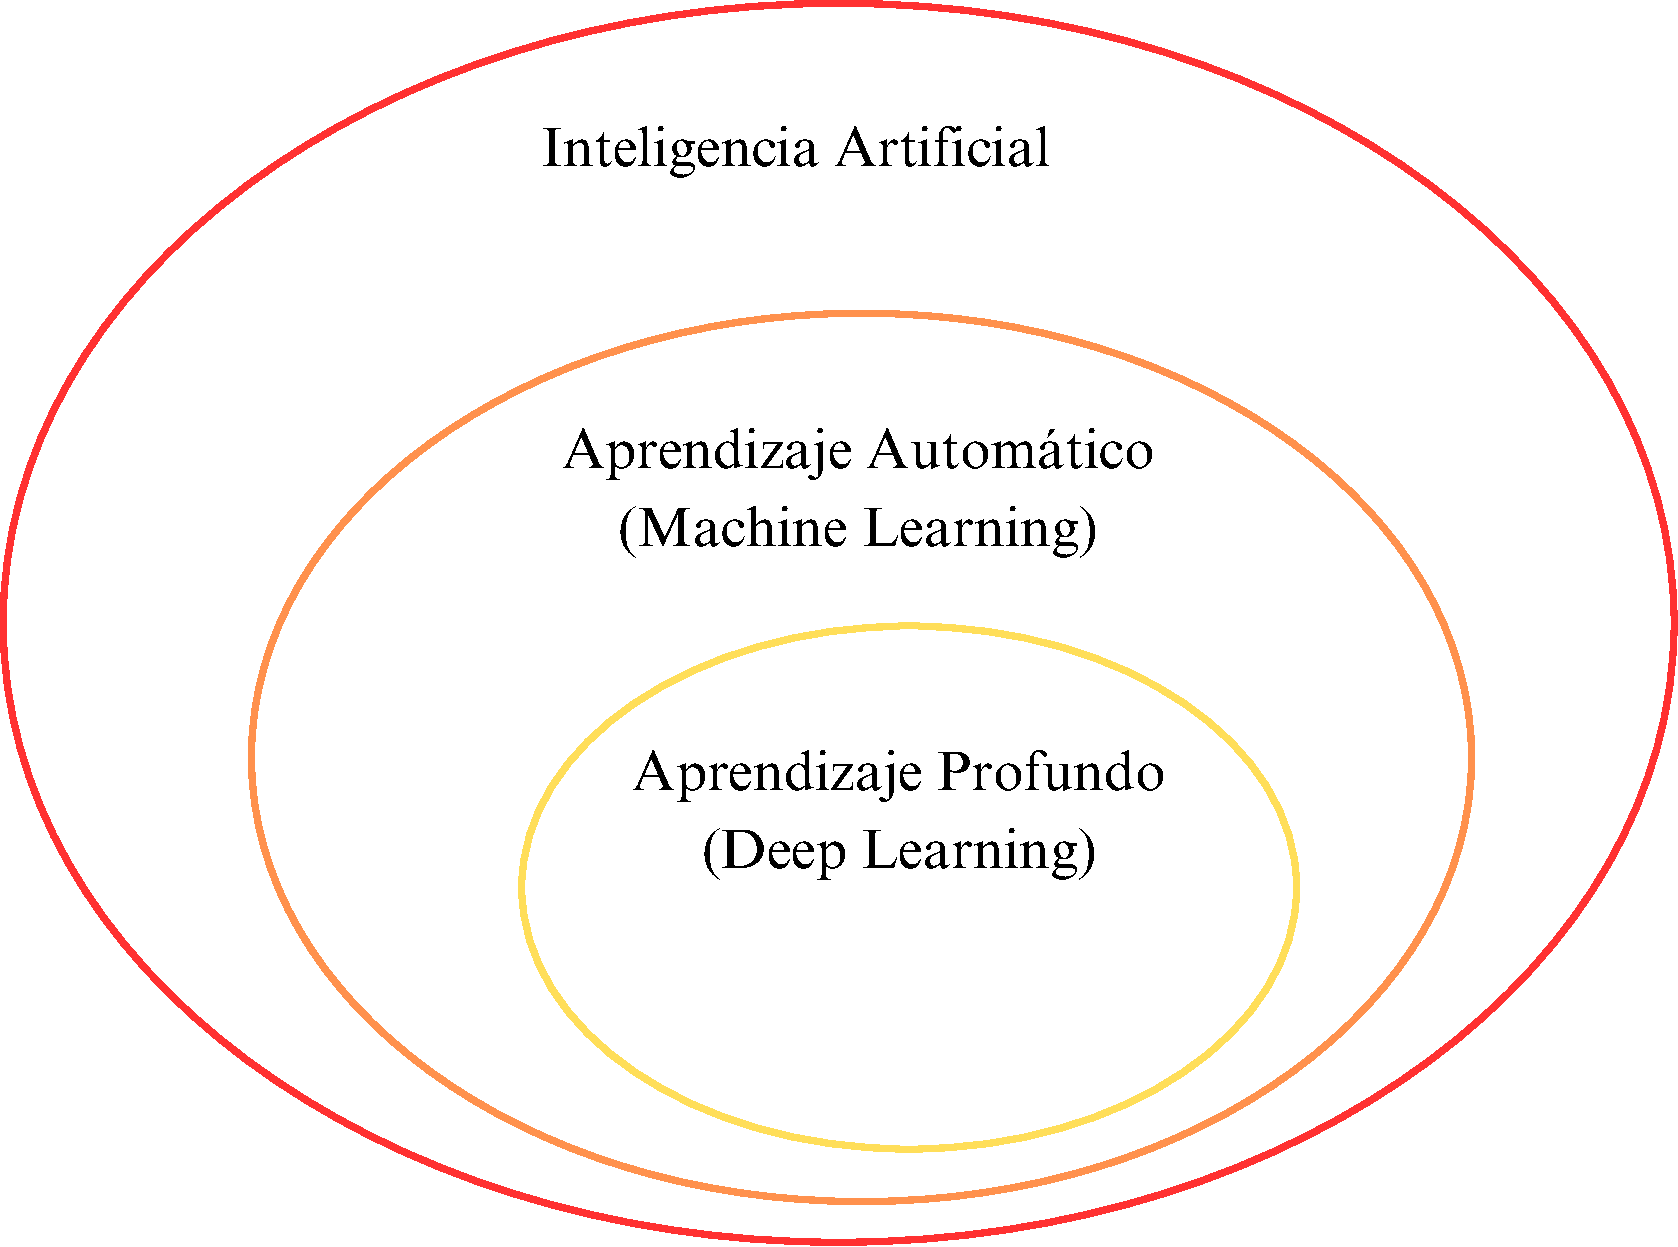
\includegraphics[width=0.5\linewidth]{Documento/Imagenes/Marco Teorico/CamposysubcamposIA.pdf}
        \caption{Campo \textit{Machine Learning} y subcampo \textit{Deep Learning} de la \textit{Inteligencia Artificial}}
        \label{fig:MLDL}
    \end{figure}

El \textbf{\textit{Machine Learning}} es un enfoque dentro de la IA que permite a las máquinas analizar y aprender de los datos mediante el uso de algoritmos sin ser programadas explícitamente para realizar una tarea. Utiliza algoritmos para reconocer patrones en grandes volúmenes de datos y hacer predicciones o tomar decisiones basadas en esos datos \cite{sanchez2020evaluacion}.  
%ref: https://uvadoc.uva.es/bitstream/handle/10324/43277/TFG-G4450.pdf?sequence=1 %

Técnicas de Machine Learning más utilizadas: 
\begin{itemize}
    \item SVM (Máquinas de Soporte Vectorial): Se usan para la clasificación de imágenes al identificar márgenes que separan diferentes clases de datos.
    \item Árboles de Decisión: Utilizados para clasificar y segmentar imágenes basándose en características específicas.
    \item k-NN (k-Nearest Neighbors): Un algoritmo de clasificación que asigna etiquetas a las imágenes según la proximidad a los ejemplos de entrenamiento.
\end{itemize}


El \textbf{\textit{Deep Learning}} es una técnica o subconjunto dentro del campo de \textit{Machine Learning} que emplea redes neuronales profundas para aprender representaciones jerárquicas de los datos, mejorando la capacidad de realizar tareas complejas como el reconocimiento de imágenes y la traducción automática \cite{avila2020plant}.
%ref: http://ricaxcan.uaz.edu.mx/jspui/bitstream/20.500.11845/1623/1/Articulo%20AMIA_%20STUDY%20AND%20COMPARISON%20OF%20OBJECTS%20DETECTION%20ALGORITHMS%20USING%20CONVOLUTIONAL%20NEURAL%20NETWORKS%20FOR%20PLANT%20DISEASES%20DETECTION%20IN%20LEAVES.pdf %
A diferencia de la IA simbólica, donde los humanos proporcionan reglas para procesar datos, en el Aprendizaje Automático los humanos solo suministran datos y las respuestas esperadas. El sistema aprende las reglas que relacionan las entradas con sus salidas, y luego puede aplicarlas a nuevos datos para generar respuestas automáticamente, sin intervención directa de los programadores. El \textit{Deep Learning} se ha convertido en la técnica predominante en visión artificial especialmente adecuada para tareas complejas como la detección de objetos en imágenes \cite{Goodfellow-et-al-2016}\cite{centeno2019deep}.
%ref: file:///C:/Users/itzel_dlz6lv9/Downloads/52%20Deep%20Learning%20autor%20Alba%20Centeno%20Franco.pdf %

La inteligencia artificial (IA) busca dotar a las máquinas de capacidades cognitivas humanas, como la percepción visual. Dentro de la IA, el aprendizaje automático (machine learning) permite a los sistemas aprender de los datos, y el aprendizaje profundo (deep learning), una subdisciplina del aprendizaje automático, utiliza redes neuronales profundas, como las CNNs, para detectar patrones complejos en grandes volúmenes de datos visuales.

Una \textbf{Red Neuronal Artificial (RNA)} es un modelo matemático inspirado en el comportamiento biológico de las neuronas y la estructura del cerebro, utilizado para resolver una amplia variedad de problemas. En una RNA, las neuronas artificiales procesan información de manera similar a las neuronas biológicas. Cada neurona recibe entradas ponderadas, las suma, y pasa el resultado a través de una función de activación. Este proceso permite que la red aprenda patrones y tome decisiones basadas en los datos que recibe\cite{centeno2019deep}.

Las neuronas en una RNA se organizan en capas que facilitan el procesamiento de la información. Las tres capas principales son:
\begin{enumerate}
    \item Capa de entrada: Recibe los datos iniciales y los transmite a la siguiente capa.
    \item Capas ocultas: Realizan el procesamiento intermedio mediante la transformación de las entradas a través de funciones de activación. Pueden ser múltiples en redes profundas.
    \item Capa de salida: Produce el resultado final del modelo, como una clasificación o predicción.
\end{enumerate}

\begin{figure}[H]
        \centering
        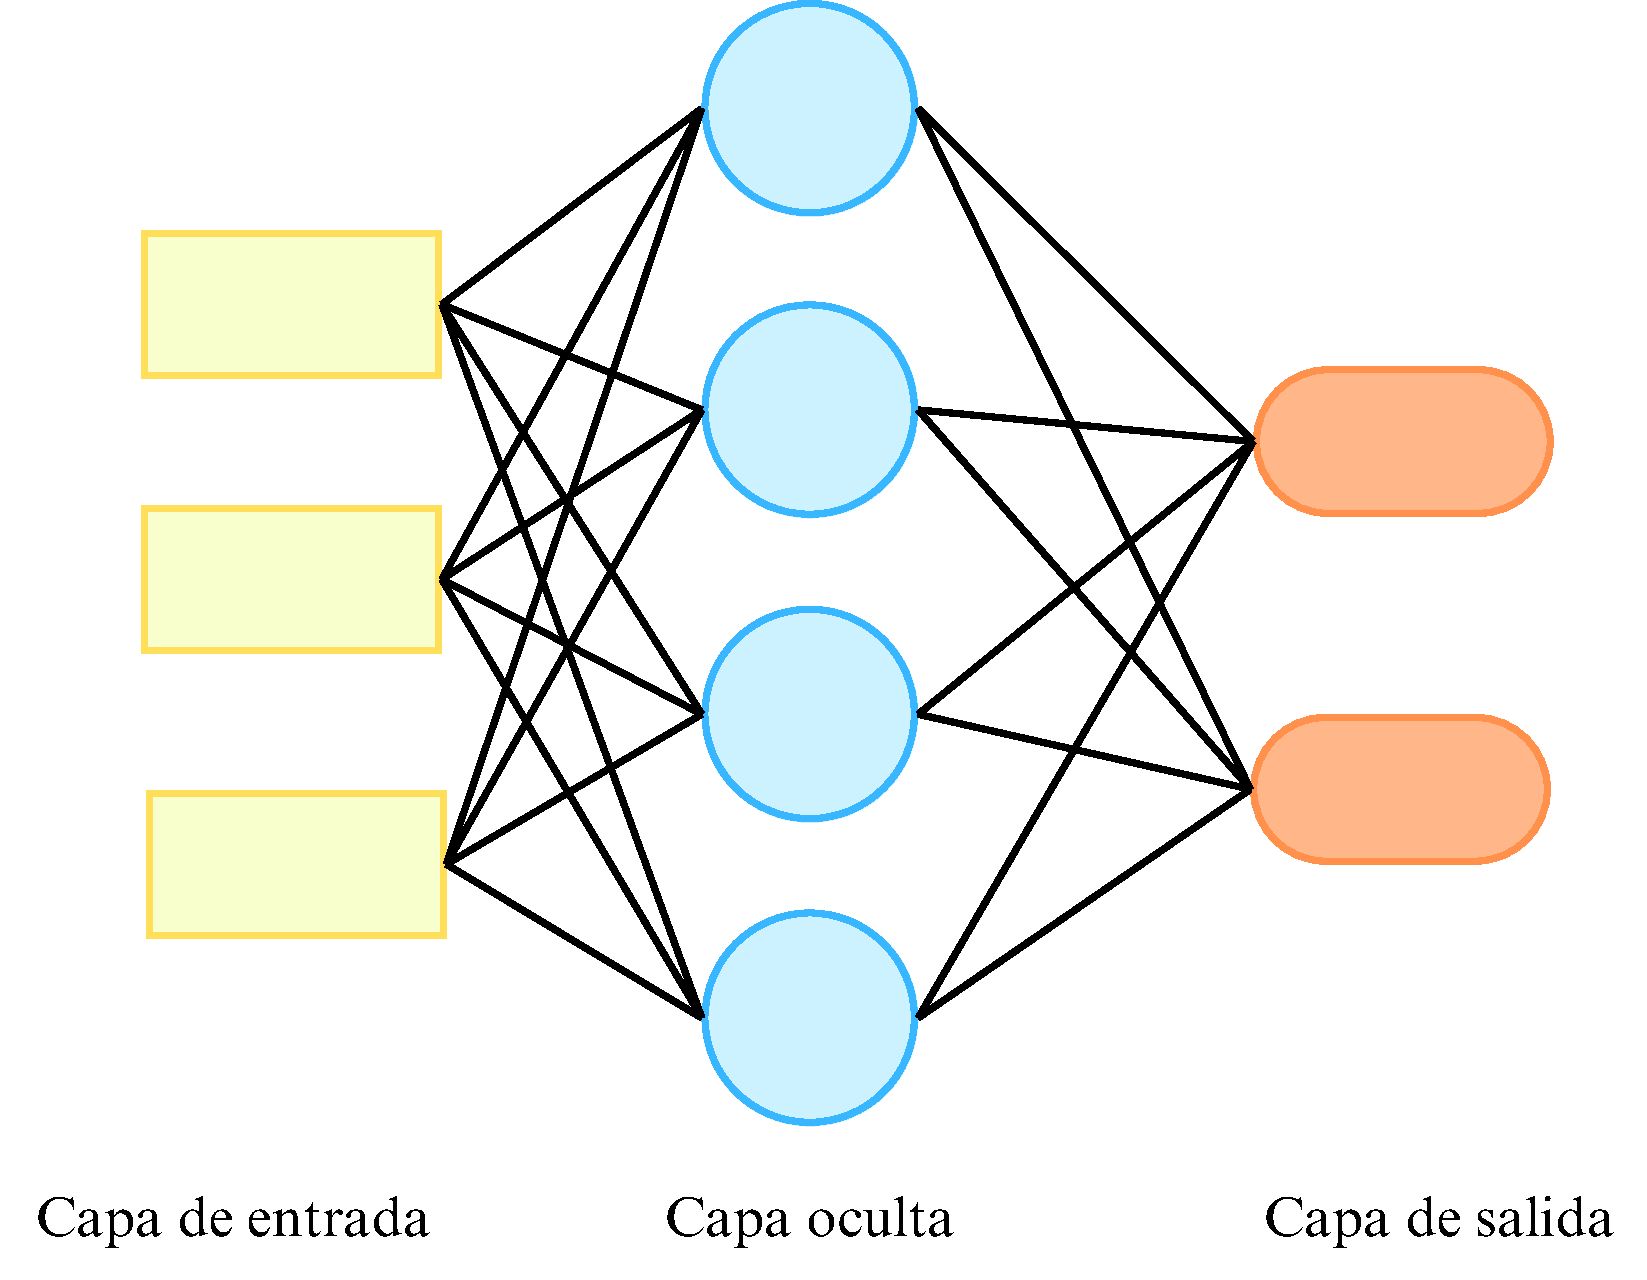
\includegraphics[width=0.6\linewidth]{Documento/Imagenes/Marco Teorico/RNA.pdf}
        \caption{Capas de una Red Neuronal Artificial}
        \label{fig:RNA}
\end{figure}

Cada neurona dentro de una capa recibe señales ponderadas de la capa anterior, las procesa y pasa el resultado a la siguiente capa. Este flujo de información permite que las redes neuronales aprendan a reconocer patrones y realizar tareas complejas.
En una RNA, los enlaces sinápticos (flechas que conectan las neuronas) indican el flujo de información entre las neuronas de diferentes capas. Estos enlaces tienen asignados pesos sinápticos, que controlan la influencia de las entradas. El número de capas de una RNA se calcula sumando las capas ocultas y la capa de salida.
En una Red Neuronal Artificial, el algoritmo o método de aprendizaje se refiere al procedimiento que asigna valores a los coeficientes sinápticos (pesos y umbral de activación). 
Existen diferentes tipos de aprendizaje en las Redes Neuronales Artificiales\cite{centeno2019deep}:
\begin{itemize}
    \item \textbf{Aprendizaje Supervisado}: La red aprende a partir de ejemplos con entradas y salidas correctas.
    \item \textbf{Aprendizaje No Supervisado}: La red aprende solo de las entradas, sin salidas correctas.
    \item \textbf{Aprendizaje Híbrido}: Combina aprendizaje supervisado en algunas capas y no supervisado en otras.
    \item \textbf{Aprendizaje por Refuerzo}: La red aprende a través de recompensas o castigos, sin ejemplos de salidas correctas.
\end{itemize}

%ref: Goodfellow, Ian, Yoshua Bengio, and Aaron Courville. Deep Learning. MIT Press, 2016.%
%ref: file:///C:/Users/itzel_dlz6lv9/Downloads/52%20Deep%20Learning%20autor%20Alba%20Centeno%20Franco.pdf %

Las redes neuronales son técnicas que pueden utilizarse tanto en \textit{Machine Learning (ML)} como en \textit{Deep Learning (DL)}. Sin embargo, la diferencia clave radica en su profundidad y capacidad de aprendizaje, en DL tenemos la disponibilidad de conjuntos de datos masivos.

La \textbf{\textit{Visión Artificial}} permite a las máquinas comprender el mundo a partir de imágenes. A través de procesos como la adquisición, el preprocesamiento, la segmentación y el reconocimiento de patrones, las máquinas pueden identificar y clasificar objetos. Esto permite automatizar tareas repetitivas de inspección, controlar la calidad de productos, realizar procesos de inspección sin contacto físico, reducir el tiempo de ciclo en procesos automatizados \cite{visionartificial}.

Se trata de deducir automáticamente la estructura y propiedades de un entorno tridimensional a partir de imágenes bidimensionales. Estas propiedades incluyen tanto aspectos geométricos (como forma, tamaño y ubicación) como materiales (como color, textura e iluminación) de los objetos \cite{visionartificialunirioja}. 

En \cite{visionporcomputador} se definen cuatro fases principales de un sistema de Visión Artificial:
\begin{itemize}
    \item \textbf{Fase sensorial}: Captura de imágenes mediante sensores.
    \item \textbf{Preprocesamiento}: Eliminación de ruido y realce de características importantes.
    \item \textbf{Segmentación}: Aislamiento de regiones de interés en la imagen mediante técnicas de umbralización, detección de bordes o clustering, permitiendo la identificación de objetos dentro de la escena.
    \item \textbf{Reconocimiento/Clasificación}: Identificación de objetos segmentados mediante análisis de características y algoritmos de aprendizaje automático
\end{itemize}

Como muestra la Figura \ref{fig:proceso_vision}, este flujo no es estrictamente secuencial sino iterativo: cuando falla la clasificación, se retrocede a etapas anteriores (segmentación o preprocesamiento), e incluso se repite la captura si se detectan artefactos irreparables en la imagen fuente \cite{visionporcomputador}.

\begin{figure}[H]
    \centering
    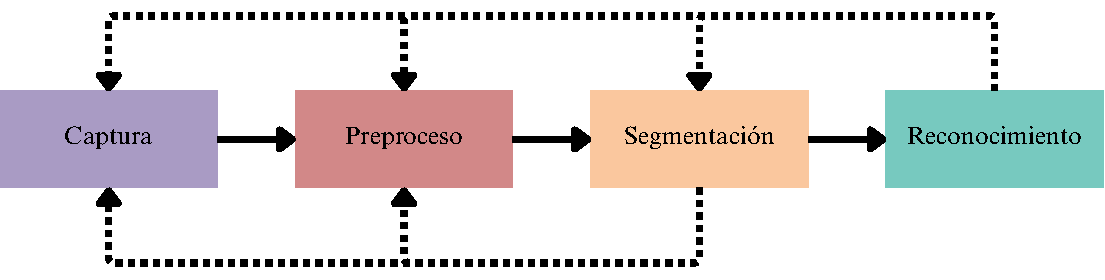
\includegraphics[width=0.8\linewidth]{Documento/Imagenes/Marco Teorico/Dig_blo_VA.pdf}
    \caption{Diagrama de bloques de las etapas típicas en un sistema de visión artificial\cite{visionporcomputador}}
    \label{fig:proceso_vision}
\end{figure}

%ref: https://publicaciones.unirioja.es/catalogo/online/VisionArtificial.pdf
%%%%%%%%%%%%%%%%%%%%%%%%%%%%%%%%
%          Tecnicas            %
%%%%%%%%%%%%%%%%%%%%%%%%%%%%%%%%


\subsection{Técnicas y Algoritmos de Visión Artificial}

El documento \cite{visionArtificial2024} presenta diversas metodologías empleadas en el procesamiento y análisis de imágenes. A continuación, se resumen los principales algoritmos y técnicas:

\begin{itemize}
    \item \textbf{Preprocesamiento de Imágenes}:
    \begin{itemize}
        \item \textbf{Filtrado espacial}: Uso de máscaras para resaltar características o reducir el ruido.
        \item \textbf{Transformaciones geométricas}: Ajustes como traslación, rotación y escalado.
        \item \textbf{Corrección de iluminación}: Mejora de la iluminación para uniformidad en los datos visuales.
    \end{itemize}

    \item \textbf{Segmentación de Imágenes}:
    \begin{itemize}
        \item \textbf{Umbralización}: Separación de objetos del fondo.
        \item \textbf{Detección de bordes}: Identificación de contornos con operadores como Sobel o Canny.
        \item \textbf{Regiones de interés (ROI)}: Aislamiento de áreas específicas para análisis detallado.
    \end{itemize}

    \item \textbf{Extracción de Características}:
    \begin{itemize}
        \item \textbf{Análisis de formas}: Cálculo de propiedades geométricas.
        \item \textbf{Textura}: Evaluación de patrones de intensidad.
        \item \textbf{Color}: Uso de la cromática para distinguir y clasificar elementos.
    \end{itemize}

    \item \textbf{Reconocimiento de Patrones}:
    \begin{itemize}
        \item \textbf{Clasificación supervisada}: Uso de algoritmos como SVM o redes neuronales.
        \item \textbf{Clasificación no supervisada}: Técnicas como clustering para agrupar datos.
    \end{itemize}

    \item \textbf{Seguimiento de Objetos}:
    \begin{itemize}
        \item \textbf{Filtros de Kalman}: Estimación de la posición y movimiento en secuencias de imágenes.
        \item \textbf{Algoritmos de correlación}: Comparación de regiones a lo largo del tiempo.
    \end{itemize}
\end{itemize}

En el Reconocimiento de Patrones, la Clasificación Supervisada es una tarea clave dentro del Aprendizaje Supervisado, donde el modelo asigna una etiqueta a cada entrada según las salidas proporcionadas durante el entrenamiento.

Dentro de las Redes Neuronales Artificiales (RNA), las \textbf{Redes Neuronales Profundas} o \textbf{\textit{Deep Neural Network(DNN)}} son fundamentales, están compuestas por múltiples capas que permiten a las máquinas aprender representaciones jerárquicas de los datos. En el caso de las imágenes, las primeras capas pueden detectar bordes simples, mientras que las capas posteriores pueden reconocer patrones más complejos, como formas o incluso objetos completos, sin intervención humana directa en el diseño de esas características\cite{centeno2019deep}.
%ref: https://www.researchgate.net/publication/277411157_Deep_Learning%

Existen diferentes redes dentro de las DNN, como las RNN y sus variantes LSTM/GRU son útiles para tareas secuenciales como reconocimiento de voz, traducción automática y escritura a mano. Las CNN se destacan en reconocimiento de imágenes, análisis de video y procesamiento de lenguaje natural. Las DBN son eficaces en recuperación de información y predicción de fallas, mientras que las DSN ayudan en reconocimiento continuo de voz y clasificación de imágenes. Las GAN son ideales para generación de imágenes y síntesis de datos, y los Transformers son fundamentales en procesamiento de lenguaje natural, traducción automática y generación de texto. Cada una de estas redes está optimizada para tareas específicas y tiene ventajas particulares en diversos campos de la inteligencia artificial\cite{centeno2019deep}.
%ref: file:///C:/Users/itzel_dlz6lv9/Downloads/52%20Deep%20Learning%20autor%20Alba%20Centeno%20Franco.pdf %

En la etapa de Segmentación en un sistema de Visión Artificial podemos encontrar la detección de objetos, es una tarea clave que busca identificar y localizar objetos dentro de una imagen, utilizando métodos como cuadros delimitadores o segmentación. Antes del deep learning, se usaban técnicas como  SIFT (Scale-Invariant Feature Transform) y HOG (Histogram of Oriented Gradients) para extraer características y comparar imágenes con plantillas de objetos. Con la llegada de las Redes Neuronales Convolucionales (CNN), este proceso se simplificó y mejoró, permitiendo la detección automática de características complejas\cite{sanchez2020evaluacion}.
%ref: https://uvadoc.uva.es/bitstream/handle/10324/43277/TFG-G4450.pdf?sequence=1%

\subsection*{Algoritmos para la detección de objetos} 

\textbf{CNN (Redes Neuronales Convolucionales)}: Las redes neuronales convolucionales (CNN, por sus siglas en inglés) son una técnica dentro del campo del aprendizaje profundo (\textit{Deep Learning}). Específicamente, son un tipo de red neuronal artificial que se utiliza para procesar datos con una estructura en forma de rejilla, como las imágenes, la diferencia fundamental entre las redes neuronales convencionales y las redes neuronales convolucionales es que estas últimas están específicamente diseñadas para que los datos de entrada sean imágenes. Son ampliamente utilizadas en tareas de clasificación, detección y segmentación de objetos\cite{centeno2019deep}\cite{sanchez2020evaluacion}\cite{iaavanzada}.

Su arquitectura se compone de múltiples capas, incluyendo capas convolucionales, capas de activación (como ReLU), capas de agrupamiento (\textbf{pooling}) y capas completamente conectadas. Las capas convolucionales aplican filtros a las imágenes para detectar características como bordes, formas y texturas, mientras que las capas profundas permiten la identificación de patrones complejos de alto nivel.
    
    \begin{figure}[H]
        \centering
        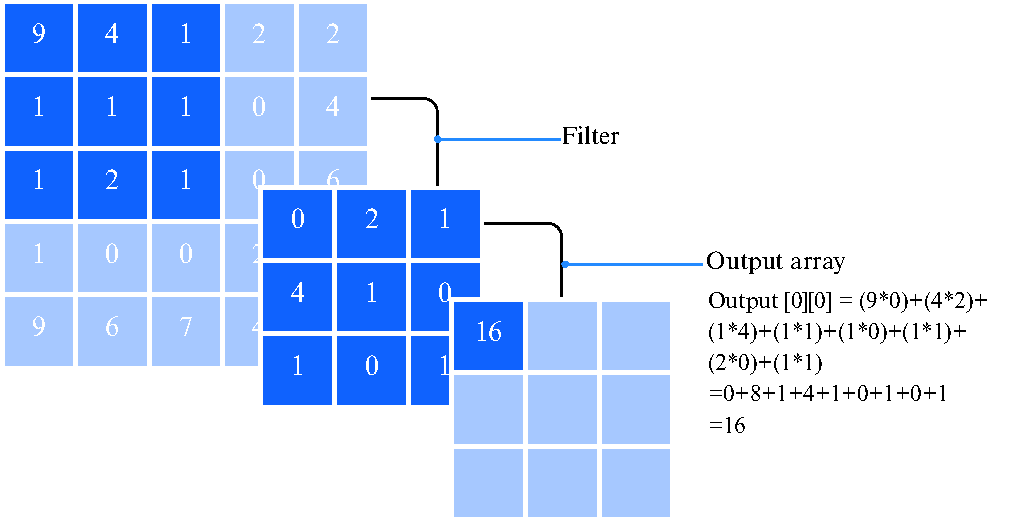
\includegraphics[width=0.8\linewidth]{Documento/Imagenes/Marco Teorico/CNN.pdf}
        \caption{Ejemplo del proceso de convolución entre una matriz de entrada y un filtro 3×3. Se ilustra el cálculo del primer elemento del mapa de características resultante (output array).}
        \label{fig:cnnIBM}
    \end{figure}
    
    Gracias a su capacidad de aprendizaje automático y a su robustez frente a variaciones en iluminación, escala o rotación, las CNN se han convertido en el estándar para muchas aplicaciones de visión por computadora con tareas complejas como el reconocimiento y la clasificación, incluyendo el reconocimiento facial, la conducción autónoma y el análisis médico por imágenes \cite{cnnIBM}.

\textbf{R-CNN}: Fue uno de los primeros modelos de detección de objetos basados en aprendizaje profundo. R-CNN es un método de detección de objetos de dos etapas que divide el proceso en dos fases: generación de propuestas de objetos y clasificación de esas propuestas. Primero, utiliza el algoritmo de búsqueda selectiva para generar alrededor de 2000 propuestas de regiones en la imagen. Luego, estas propuestas son procesadas por una red neuronal convolucional (CNN) para extraer características de cada una. Después de esto, se utiliza un clasificador SVM para identificar los objetos en cada región. Aunque R-CNN representó un avance importante en la detección de objetos basada en aprendizaje profundo, su principal desventaja es la lentitud en el proceso, debido a la redundancia en el cálculo de características a través de un gran número de propuestas de regiones superpuestas, lo que hace que el modelo sea muy lento, incluso con aceleración por GPU\cite{wang2024yolosurvey}\cite{sapkota2025yolo}.

\textbf{Fast R-CNN}: Mejoró la eficiencia de R-CNN al integrar la extracción de características y la clasificación en un solo paso, reduciendo el tiempo de procesamiento al eliminar los cálculos redundantes. Esto permitió una detección más rápida y eficiente \cite{sapkota2025yolo}.

\textbf{Faster R-CNN}: Es la evolución de R-CNN y Fast R-CNN. Comenzó con "Rich feature hierarchies for accurate object detection and semantic segmentation" (R-CNN), utilizando un algoritmo de búsqueda selectiva para proponer posibles regiones de interés y una CNN estándar para clasificarlas y ajustarlas. Fast R-CNN, introdujo "Region of Interest Pooling", que permitió compartir cálculos costosos, haciendo el modelo mucho más rápido. Finalmente, Faster R-CNN propuso el primer modelo de esta arquitectura, mejorando la eficiencia en la detección de objetos\cite{centeno2019deep}\cite{sanchez2020evaluacion}.

\textbf{SSD (Single Shot MultiBox Detector)}: SSD realiza tanto la localización como la clasificación de objetos en un solo paso de la red. Utiliza una técnica llamada "MultiBox" para la regresión del cuadro delimitador, haciendo que la red clasifique y detecte objetos de manera eficiente. Mejoró la detección al utilizar cajas delimitadoras predeterminadas de diversas escalas y proporciones, y predecir las puntuaciones de los objetos y ajustar las formas de las cajas. Utiliza mapas de características multiescala para manejar objetos de diferentes tamaños, eliminando la necesidad de un paso separado de generación de propuestas y mejorando el rendimiento en la detección de objetos pequeños. Revolucionó la detección de objetos al simplificar el proceso con un enfoque de una sola etapa, inspirando desarrollos posteriores en los modelos YOLO. A diferencia de los modelos de dos etapas como R-CNN, que dependen de una etapa de propuesta de región antes de la detección real, SSD y, por extensión, las variantes de YOLO, realizan la detección y clasificación en una sola pasada por la imagen. Este cambio de paradigma mejora el proceso de detección al eliminar pasos intermedios, lo que facilita una detección de objetos más rápida y eficiente, adecuada para aplicaciones en tiempo real. La arquitectura de SSD, que los modelos YOLO han adaptado, utiliza múltiples mapas de características a diferentes resoluciones para detectar objetos de varios tamaños, empleando una variedad de cajas ancla en cada ubicación del mapa de características para mejorar la precisión de la localización.

YOLO incorpora los principios arquitectónicos de SSD para mejorar las capacidades de detección en tiempo real mediante una mejor extracción de características utilizando capas de atención multi-cabeza. Esta adopción de la metodología SSD mejora significativamente la velocidad de procesamiento y la precisión de detección de modelos como YOLOv8, YOLOv9 y YOLOv10, haciéndolos ideales para la detección rápida y confiable de objetos en entornos con recursos limitados. El mecanismo eficiente de detección de un solo paso, que clasifica y localiza objetos directamente, destaca la evolución continua de la serie YOLO para cumplir con los requisitos de precisión y velocidad en diversos escenarios del mundo real\cite{sapkota2025yolo}\cite{sanchez2020evaluacion}.

\textbf{YOLO (You Only Look Once)}: Es un algoritmo de detección de objetos que se distingue por su capacidad para realizar esta tarea en un solo paso, a diferencia de métodos previos como R-CNN que emplean un pipeline de múltiples etapas. Al tomar una imagen de entrada y pasarla a través de una red neuronal convolucional (CNN), YOLO predice simultáneamente las coordenadas de las cajas delimitadoras y las clases de los objetos. Este enfoque simplifica el proceso de detección y mejora su eficiencia, abordando la tarea como un único problema de regresión.
Este enfoque permite que YOLO es extremadamente rápido, lo que lo convierte en una opción ideal para aplicaciones en tiempo real, como vehículos autónomos, vigilancia de video y robótica. Además, ha mejorado con el tiempo, ofreciendo mayor precisión, especialmente en la detección de objetos pequeños y en diferentes escalas, sin sacrificar su rapidez.
Si bien su principal ventaja es la detección en tiempo real, también se emplea en áreas donde la velocidad no es crítica. En campos como la agricultura y la medicina, se prioriza la precisión y fiabilidad del modelo, ayudando en tareas como la clasificación de cultivos o la detección de enfermedades, donde la rapidez y procesamiento en tiempo real no es un factor esencial\cite{sanchez2020evaluacion}\cite{terven2023yolo}.

Las versiones de YOLO para la detección de objetos, destacando sus innovaciones clave, son\cite{sapkota2025yolo}\cite{terven2023yolo}:

\begin{itemize}
     
    \item \textbf{YOLOv1 (2016):} Introdujo la detección de objetos en tiempo real con una única red neuronal convolucional (CNN), permitiendo realizar la detección en un solo paso. Fue revolucionario en cuanto a velocidad, pero presentaba limitaciones en la precisión de localización.
    \textbf{Arquitectura:} 24 capas convolucionales, 2 capas completamente conectadas. Utiliza Leaky ReLU - ativación, última capa - activación lineal. Backbone: Darknet24, AP(\%): 63.4.
    
    \item \textbf{YOLOv2/YOLO9000 (2017):} Mejoró la precisión con la introducción de anclajes (anchor boxes) y normalización por lotes, lo que aumentó la estabilidad y rendimiento del modelo. También adoptó una arquitectura completamente convolucional, mejorando la flexibilidad y desempeño. La arquitectura de YOLOv2 mantiene la estructura de YOLOv1, pero con mejoras clave. 
    \textbf{Arquitectura:} 19 capas convolucionales y cinco capas de max pooling capas convolucionales, implementación de anchor boxes para precision. Utiliza Leaky ReLU - ativación, última capa - activación lineal. Backbone: Darknet19, AP(\%): 78.6.
    
    \item \textbf{YOLOv3 (2018):} Incorporó una arquitectura más profunda (Darknet-53) y la capacidad de realizar predicciones multi-escala, mejorando la detección de objetos pequeños y en diferentes escalas. Se enfocó en equilibrar precisión y velocidad sin sacrificar rendimiento. YOLOv3 introdujo tres variantes principales, cada una diseñada para equilibrar el tamaño del modelo y el rendimiento: YOLOv3-spp (Small), Standard y YOLOv3-tiny (Tiny), adaptadas a diferentes compensaciones entre velocidad y precisión.  Este modelo introduce predicción multiescala, utilizando tres diferentes tamaños de grilla para detectar objetos en distintas escalas. El neck es una combinación de PANet (Path Aggregation Network), lo que mejora la fusión de características a través de diferentes niveles. El head predice las cajas y clases en tres escalas diferentes.
    \textbf{Arquitectura:} 53 capas convolucionales y residual connections para facilitar el flujo de gradientes y mejorar el aprendizaje profundo; utiliza Leaky ReLU - ativación, última capa - activación lineal. Backbone: Darknet53; AP(\%):36.2.
    
    \item \textbf{YOLOv4 (2020):} Implementó CSPNet, la función de activación Mish y técnicas avanzadas como SPP (Spatial Pyramid Pooling) y PANet (Path Aggregation Network), lo que mejoró la precisión y eficiencia computacional sin sacrificar la velocidad. YOLOv4 introdujo cuatro variantes principales: la versión estándar, YOLOv4-CSP, que incorpora redes Cross-Stage Partial (CSP) para mejorar el rendimiento y reducir los costos computacionales; YOLOv4x-mish, que utiliza la función de activación Mish para mejorar la precisión mientras mantiene la eficiencia; y YOLOv4-tiny, una versión ligera optimizada para aplicaciones en tiempo real y dispositivos de borde, sacrificando algo de precisión por velocidad. YOLOv4 utiliza el backbone CSPDarknet-53, con Cross-Stage Partial connections que permiten una mayor eficiencia computacional. Esta versión introduce técnicas avanzadas como Mish activation, DropBlock regularization, y Bag of Freebies (BoF) para mejorar la precisión sin aumentar la carga computacional. El neck está compuesto por PANet para una mejor fusión de características multiescala, mientras que el head optimiza la salida usando técnicas como Label Smoothing y CutMix.   
    \textbf{Arquitectura:} 53 capas convolucionales y residual connections para facilitar el flujo de gradientes y mejorar el aprendizaje profundo. Backbone: CSPDarknet-53; AP(\%):43.5.
   
     \item \textbf{Scaled-YOLOv4 (2020):} Utilizó un enfoque de escalado para generar modelos más grandes y pequeños según las necesidades de la aplicación. Scaled-YOLOv4 logró un AP de 56\% en MS COCO con la versión más grande, mientras que su versión más pequeña, YOLOv4-tiny, se ejecutó a 440 FPS en un RTX2080Ti. Mejoró la detección de objetos al eliminar los pasos de preentrenamiento y entrenar desde cero, lo que permitió obtener resultados de alta calidad. Introdujo mejoras clave como CSPNet en PAN, modelos escalables (P5, P6, P7) para dispositivos de borde, y técnicas de escala de modelos combinada para optimizar la eficiencia. Además, utilizó una arquitectura amigable con el hardware y resolvió la inconsistencia de resolución entre modelos preentrenados y datos de entrada mediante un método de escalado eficiente. Estas mejoras le permitieron alcanzar la más alta precisión y velocidad de inferencia en su categoría.
     \textbf{Arquitectura:} Backbone: CSPDarknet; AP(\%):56.0.
     
    \item \textbf{YOLOv5 (2020):} Aunque no es una versión oficial de la serie, se destacó por su facilidad de uso, optimización en Pytorch y un excelente rendimiento en tiempo real. Ofrece versiones escalables (como YOLOv5n, YOLOv5s, etc.) para adaptarse a diferentes necesidades. Introdujo cinco variantes principales para satisfacer diversas necesidades de rendimiento: YOLOv5s (pequeña), optimizada para velocidad y eficiencia en entornos con recursos limitados; YOLOv5m (media), ofreciendo un balance entre velocidad y precisión; YOLOv5l (grande), diseñada para mayor precisión a costa de recursos; YOLOv5x (extra grande), enfocada en la precisión de alto nivel para hardware potente; y YOLOv5n (nano), una versión ligera adaptada para inferencia rápida y bajas demandas computacionales, ideal para aplicaciones en tiempo real y dispositivos de borde.
    \textbf{Arquitectura:} Backbone: ModifiedCSPv7; AP(\%):55.8.
     
    \item \textbf{PP-YOLO (2020):} Basado en YOLOv3, mejoró con aumentos como Mixup y distorsión de colores, logrando un rendimiento sólido en tiempo real. Se mejora sobre YOLOv3, utilizando diversas técnicas de entrenamiento de YOLOv4, además de añadir métodos como CoordConv [39], Matrix NMS [40], y un mejor modelo preentrenado de ImageNet.
    \textbf{Arquitectura:} Backbone: ResNet50-vd; AP(\%):45.9.
    
    \item \textbf{PP-YOLOv2 (2021):} Mejoró PP-YOLO con un cambio de backbone de ResNet50 a ResNet101 y la implementación de una red de agregación de rutas (PAN) en lugar de FPN.  Introduce además el CSPPAN de YOLOv4 escalado y otros mecanismos.
    \textbf{Arquitectura:} Backbone: ResNet50-vd; AP(\%):50.3.
    
    \item \textbf{YOLOR (2021):} Introdujo un enfoque de aprendizaje multitarea, donde se crea un solo modelo para diversas tareas como clasificación, detección y estimación de poses. Utiliza el conocimiento implícito de las redes neuronales para mejorar la eficiencia en múltiples tareas.
    \textbf{Arquitectura:} Backbone: CSPDarknet; AP(\%):55.4.
    
    \item \textbf{YOLOX (2021):} Revertió a una arquitectura sin anclajes y mejoró la precisión mediante center sampling y un head desacoplado para separar las tareas de clasificación y localización. Utilizó aumentaciones fuertes como MixUp y Mosaic, lo que aumentó el AP en 2.4 puntos. 
    \textbf{Arquitectura:} Backbone:  ResNet50-vd; AP(\%):50.3.
    
    \item \textbf{PP-YOLOE (2022):} Mejoró sobre PP-YOLOv2 utilizando una arquitectura sin anclajes y un nuevo backbone y neck con RepResBlocks. Implementó un aprendizaje de alineación de tareas (TAL) y una pérdida focal Varifocal (VFL). Realiza cambios importantes, modificando RepVGG y diseñando el CSPRepResStage, además de usar regresión de cajas delimitadoras en el proceso de regresión basado en distribución de TOOD. 
    \textbf{Arquitectura:} Backbone: ModifiedCSPv5; AP(\%):51.2.

    \item \textbf{YOLOv6 (2020):}  Introdujo un detector sin anclajes y un backbone basado en EfficientRep, optimizado para eficiencia. Mejoró las pérdidas de clasificación y regresión y utilizó auto-destilación para optimizar la precisión. Implementó un esquema de cuantización para acelerar el proceso sin sacrificar precisión, y fue diseñado para dispositivos con bajos recursos. Las variantes incluyen: YOLOv6 (precisión y velocidad equilibradas), YOLOv6-Nano (optimizado para velocidad en tiempo real), y YOLOv6-Tiny (inferencias rápidas en hardware limitado). RepVGG + QAT (Quantization Aware Training).
    \textbf{Arquitectura:} Backbone: EfficientRep; AP(\%):52.5.

    \item \textbf{YOLOv7 (2022):} Superó a otros detectores en velocidad y precisión, introduciendo la E-ELAN para un aprendizaje eficiente y un modelo de escalado adaptativo. Implementó RepConv para mejorar la eficiencia de las convoluciones y YOLOR para mejor generalización. Sus variantes son: YOLOv7 (equilibrio entre velocidad y precisión), YOLOv7-X (mayor rendimiento, más recursos), y YOLOv7-Tiny (ligero para aplicaciones en tiempo real).
    \textbf{Arquitectura:} Backbone: RepConvN; AP(\%):56.8.
    
    \item \textbf{DAMO-YOLO (2022):} Introdujo la búsqueda de arquitectura neuronal (NAS) y optimizó la arquitectura con un neck eficiente llamado Efficient-RepGFPN. Implementó un enfoque de destilación de conocimiento para mejorar la precisión. 
    \textbf{Arquitectura:} Backbone:   MAE-NAS; AP(\%):50.0.
    
    \item \textbf{YOLOv8 (2023):}  Presenta una arquitectura más eficiente, técnicas de entrenamiento mejoradas y soporte para conjuntos de datos más grandes. Su implementación fácil de usar en PyTorch lo hace accesible tanto para la investigación como para la producción, que optimiza el proceso de NMS (Supresión de No Máximos), mejora la precisión y la velocidad, además de implementar una arquitectura sin anclajes, facilitando su rendimiento y flexibilidad. También utiliza aumentos de datos avanzados y técnicas de optimización para mejorar la generalización del modelo. Tiene cuatro variantes YOLOv8-S, optimizada para inferencia rápida en dispositivos de borde con algunas compensaciones en precisión; YOLOv8-M, equilibrando precisión y velocidad para tareas generales; YOLOv8-L, priorizando la precisión a costa de la demanda computacional; y YOLOv8-Tiny, una versión ligera para aplicaciones en tiempo real.
    \textbf{Arquitectura:} Backbone: YOLOv8; AP(\%):53.8.

    \item \textbf{YOLOv9 (2024):} Propone el concepto de información de gradiente programable (PGI) para enfrentar los diversos cambios requeridos por las redes profundas para lograr múltiples objetivos. PGI puede proporcionar información completa de entrada para la tarea objetivo para calcular la función objetivo, de modo que se pueda obtener información de gradiente confiable para actualizar los pesos de la red. Además, se diseñó una nueva arquitectura de red ligera, Generalized Efficient Layer Aggregation Network (GELAN), basada en la planificación de rutas de gradiente. 
    \textbf{Arquitectura:} Backbone:  ResNet50-vd; AP(\%):50.3.

    \item \textbf{YOLOv10 (2024):} Introduce un enfoque novedoso para la detección de objetos en tiempo real, abordando las limitaciones tanto del postprocesamiento como de la arquitectura del modelo en versiones anteriores de YOLO. Al eliminar la supresión de no máximos (NMS) y optimizar componentes clave del modelo, ofrece mejoras significativas en eficiencia y rendimiento. Esta versión introduce seis variantes distintas: YOLOv10-N, YOLOv10-S, YOLOv10-M, YOLOv10-B, YOLOv10-L y YOLOv10-X. Es destacable que YOLOv10-N y YOLOv10-S presentan las latencias más bajas, de 1.84 ms y 2.49 ms, respectivamente, lo que los hace altamente adecuados para aplicaciones que requieren baja latencia. YOLOv10-X logra el mAP más alto de 54.4\% y una latencia de 10.70 ms, reflejando una mejora equilibrada tanto en precisión como en velocidad de inferencia.

    \item \textbf{YOLOv11 (2024): } Avance en la detección de objetos, por su arquitectura sofisticada de backbone y neck para una mejor extracción de características. Optimiza la velocidad y eficiencia mientras mantiene una alta precisión. Equilibra precisión y eficiencia computacional, siendo adecuado para diversas aplicaciones, desde sistemas embebidos hasta implementaciones a gran escala. Tiene cinco variantes: YOLOv11n, YOLOv11s, YOLOv11m, YOLOv11L y YOLOv11x, basadas en la profundidad de la red.

    \item \textbf{YOLOv12 (2025):} Enfoque centrado en la atención. Introduce el módulo de Atención de Área (A2) y Redes de Agregación de Capa Eficiente Residual (R-ELAN) para un procesamiento mejorado de características. Utilizando estos cambios arquitectónicos,logra un rendimiento de vanguardia mientras mantiene las capacidades de detección en tiempo real. Sus variantes YOLOv12-N logró un mAP del 40.6\% con una latencia de inferencia de 1.64 ms en una GPU T4, superando a YOLOv10-N y YOLOv11-N por 2.1 mAP con una velocidad comparable. Mejor definición de contornos de objetos y activación de primeros planos en comparación con sus predecesores.
    
\end{itemize}

\subsection*{Metricas de detección de objetos}
\subsubsection*{mAP}
La Precisión Promedio (AP), tradicionalmente llamada Precisión Promedio Media (mAP), es la métrica comúnmente utilizada para evaluar el rendimiento de los modelos de detección de objetos. Mide la precisión promedio a través de todas las categorías, proporcionando un valor único para comparar diferentes modelos. 

En YOLOv1 y YOLOv2, el conjunto de datos utilizado para el entrenamiento y la evaluación fue PASCAL VOC 2007, y VOC 2012. Sin embargo, desde YOLOv3 en adelante, el conjunto de datos utilizado es Microsoft COCO (Common Objects in Context). La AP se calcula de manera diferente para estos conjuntos de datos. 

La métrica AP se basa en las métricas de precisión y recall, manejando múltiples categorías de objetos y utilizando la Intersección sobre Unión (IoU) para definir predicciones positivas.

\begin{itemize}
    \item Precisión y Recall: La precisión mide la exactitud de las predicciones positivas, mientras que el recall mide la proporción de objetos reales detectados. Hay un compromiso entre ambas, ya que aumentar el recall puede disminuir la precisión. La AP balancea estos factores utilizando la curva precisión-recall, que evalúa la precisión para diferentes umbrales de confianza.
    
    \item Manejo de múltiples categorías: Para evaluar el rendimiento en múltiples categorías de objetos, la AP calcula la precisión promedio de cada categoría y luego promedia estos valores, proporcionando una evaluación más completa del modelo.
    
    \item Intersección sobre Unión (IoU): IoU mide la superposición entre las cajas delimitadoras predichas y las reales, y se utiliza para evaluar la calidad de la localización de los objetos. El conjunto de datos COCO considera múltiples umbrales de IoU para evaluar el rendimiento del modelo en diferentes niveles de precisión en la localización.
\end{itemize}

La AP se calcula de manera diferente en los conjuntos de datos VOC y COCO:

\textbf{VOC}: Para calcular la AP en VOC (20 categorías de objetos), se sigue este proceso:
\begin{enumerate}
    \item Calcular la curva de precisión-recall variando el umbral de confianza.
    \item Calcular la precisión promedio de cada categoría usando una interpolación de 11 puntos.
    \item Promediar las APs de todas las categorías para obtener la AP final.
\end{enumerate}

\textbf{COCO}: Para COCO (80 categorías de objetos), se utiliza un método más complejo:

\begin{enumerate}
    \item Calcular la curva de precisión-recall variando el umbral de confianza.
    \item Calcular la precisión promedio usando 101 umbrales de recall.
    \item Calcular la AP en diferentes umbrales de IoU (de 0.5 a 0.95 con un paso de 0.05).
    \item Promediar las APs de las 80 categorías para cada umbral de IoU.
    \item Calcular el AP general promediando los resultados de todos los umbrales de IoU.
\end{enumerate}

La diferencia en el cálculo de AP hace difícil comparar el rendimiento entre los conjuntos de datos. El estándar actual usa COCO AP debido a su evaluación más detallada en diferentes niveles de IoU.

\textbf{Supresión de No Máximos (NMS)}:
La NMS es una técnica de postprocesamiento que reduce las cajas delimitadoras superpuestas y mejora la calidad de la detección:

\begin{itemize}
    \item Se filtran las cajas predichas usando un umbral de confianza.
    \item Se ordenan las cajas por sus puntajes de confianza en orden descendente.
    \item Se selecciona la caja con el puntaje más alto y se eliminan las cajas restantes si su IoU con la seleccionada excede un umbral predefinido.
\end{itemize}

\textbf{Backbone}: Es responsable de extraer características útiles de la imagen de entrada. Típicamente es una red neuronal convolucional (CNN) entrenada en una tarea de clasificación de imágenes a gran escala, como ImageNet. El backbone captura características jerárquicas en diferentes escalas: características de bajo nivel (como bordes y texturas) en las primeras capas, y características de alto nivel (como partes de objetos e información semántica) en las capas más profundas.

\textbf{Neck}: Es un componente intermedio que conecta el backbone con el head. Su función es agregar y refinar las características extraídas por el backbone, mejorando la información espacial y semántica a través de diferentes escalas. El neck puede incluir capas convolucionales adicionales, redes piramidales de características (FPN), o mecanismos similares para mejorar la representación de las características.

\textbf{Head}: Es el componente final del detector de objetos. Se encarga de realizar las predicciones basadas en las características proporcionadas por el backbone y el neck. Normalmente consiste en una o más subredes específicas para tareas como clasificación, localización y, más recientemente, segmentación de instancias y estimación de poses. El head procesa las características proporcionadas por el neck, generando predicciones para cada objeto candidato. Finalmente, un paso de postprocesamiento, como la supresión de no máximos (NMS), filtra las predicciones superpuestas y retiene solo las detecciones más confiables.

En los modelos YOLO, las arquitecturas se describen utilizando estas tres partes: backbone, neck y head.


% refpara yolo: https://uvadoc.uva.es/bitstream/handle/10324/43277/TFG-G4450.pdf?sequence=1
%file:///C:/Users/itzel_dlz6lv9/Downloads/2304.00501v1.pdf
%https://arxiv.org/pdf/2406.19407
    




%%%%%%%%%%%%%%%%%%%%%%%%%%%%


\subsection{Cámaras}

Su función es capturar la imagen proyectada en el sensor, vía las ópticas, para poder transferirla a un sistema electrónico. Las cámaras utilizadas en visión artificial requieren de una serie de características que permitan el control del disparo de la cámara para capturar piezas que pasan por delante de ella  en la posición requerida.


La visión artificial permite identificar y clasificar residuos sólidos en cuerpos de agua de forma automatizada, superando las limitaciones de los métodos manuales. Mediante algoritmos avanzados, como redes neuronales, se procesan imágenes para detectar patrones asociados a contaminantes. Esto complementa los datos de los sensores, proporcionando una visión integral del estado del agua y el impacto de los residuos en los ecosistemas.

%%%%%%%%%%%%%%%%%%%%%%%%%%%%%%%%%%%%%
%       SECCION PAGINA WEB          %
%%%%%%%%%%%%%%%%%%%%%%%%%%%%%%%%%%%%%

\section{Página Web}
%referencia: https://www.redalyc.org/pdf/421/42118510.pdf
Una página web es un archivo creado en el lenguaje HTML (HyperText Markup Language), diseñado para ser accesible a través de un servidor de Internet mediante un navegador. Su propósito es proporcionar información o servicios a una comunidad específica o al público en general \cite{redalyc2006}.

Cada página web constituye una unidad de información independiente, identificada por una dirección única (URL) dentro de un sitio web. Puede contener elementos como texto, imágenes, gráficos, videos y enlaces a otros documentos o páginas. Aunque el término "página web" a menudo se confunde con "sitio web", este último se refiere al conjunto completo de páginas relacionadas bajo un dominio principal.

% Una aplicación web (web-based application) es un tipo especial de aplicación cliente/servidor, donde tanto el cliente (el navegador, explorador o visualizador1) como el servidor (el servidor web) y el protocolo mediante el que se comunican (HTTP) están estandarizados y no han de ser creados por el programador de aplicaciones\cite{lujan2011programacion}.
La página web permitirá centralizar y presentar de forma clara y accesible los datos recopilados sobre calidad del agua y detección de residuos sólidos. Facilitará la consulta dinámica por parámetros, fechas o ubicaciones, fomentando la transparencia, la conciencia pública y la participación ciudadana. Además, asegurará la disponibilidad de información para un público amplio, sin requerir software especializado, y será adaptable para futuras mejoras y funcionalidades.


\section{Servidor}
En el ámbito de la informática, un servidor se define como un sistema (hardware, software o ambos) que provee recursos, datos o servicios a otros dispositivos, denominados clientes, bajo el modelo de arquitectura cliente-servidor \cite{Espana2003, Britannica2024}. Sus características esenciales incluyen:

\begin{itemize}
    \item \textbf{Alta disponibilidad}: Operación continua para garantizar acceso ininterrumpido \cite{Stanek2014}.
    \item \textbf{Escalabilidad}: Capacidad de manejar múltiples solicitudes simultáneas gracias a hardware especializado (ej. CPUs multinúcleo, almacenamiento RAID) \cite{Mancera2015}.
    \item \textbf{Seguridad}: Implementación de firewalls, encriptación y control de acceso \cite{Espana2003}.
\end{itemize}

Los servidores se clasifican según su función, destacando:
\begin{itemize}
    \item \textbf{Servidores web}: Distribuyen contenido mediante protocolos como HTTP (Apache, Nginx).
    \item \textbf{Servidores de bases de datos}: Gestionan información estructurada (SQL Server, Oracle).
    \item \textbf{Servidores virtuales}: Simulan servidores físicos para optimizar recursos \cite{Stanek2014}.
\end{itemize}

La arquitectura cliente-servidor puede implementarse mediante dos modelos de despliegue principales:
\begin{itemize}
    \item \textbf{Servidores locales (on-premise)}: Infraestructura física instalada y mantenida dentro de la organización, con control total sobre hardware y datos \cite{Mullins2012}.
    
    \item \textbf{Servidores en la nube}: Infraestructura virtualizada proporcionada por terceros, accesible mediante internet, con escalabilidad bajo demanda \cite{Mell2011}.
\end{itemize}

\section{Base de Datos}

Una base de datos o banco de datos, también conocida como DB (Database), BBDD o BD, es un conjunto estructurado de datos relacionados entre sí, que se almacenan de forma sistemática para su fácil acceso, gestión y actualización. Su función principal es permitir el almacenamiento organizado de grandes volúmenes de información para su posterior consulta, modificación o análisis. Las bases de datos son fundamentales en sistemas que requieren una interacción fluida con aplicaciones, ya que permiten almacenar información dinámica que puede actualizarse en tiempo real.

Además de almacenar datos, las bases de datos también permiten mantener la integridad y la consistencia de los mismos mediante restricciones y reglas definidas en su diseño. Una base de datos bien diseñada no solo mejora el rendimiento de las consultas, sino que también optimiza la toma de decisiones basada en datos confiables.

\subsection{Tipos de Base de Datos}

Existen distintos tipos de bases de datos, cada una adecuada a diferentes necesidades según el tipo, el volumen y la velocidad de los datos que se manejan. Entre los principales tipos, destacan:

\begin{itemize}
    \item \textbf{MySQL:} Sistema de gestión de bases de datos relacional con licencia GPL. Es popular por su rapidez y facilidad de uso, aunque no está optimizado para el manejo de grandes volúmenes de datos empresariales.
    
    \item \textbf{PostgreSQL y Oracle:} Son sistemas de gestión de bases de datos robustos, altamente escalables y con soporte para operaciones complejas. Se utilizan comúnmente en aplicaciones empresariales, sistemas financieros y plataformas que requieren alta disponibilidad.
    
    \item \textbf{Microsoft Access:} Herramienta de base de datos de escritorio desarrollada por Microsoft. Se utiliza principalmente para aplicaciones locales o pequeñas bases de datos individuales, generando archivos .mdb.
    
    \item \textbf{Microsoft SQL Server:} Plataforma de base de datos relacional desarrollada por Microsoft, ideal para aplicaciones empresariales que requieren manejar grandes volúmenes de datos de forma segura y eficiente.
\end{itemize}

\subsection{Modelos de Base de Datos}

Las bases de datos pueden clasificarse según su modelo lógico:

\begin{itemize}
    \item \textbf{Bases de datos relacionales (RDB):} Organizan los datos en tablas con filas y columnas. Son las más utilizadas tradicionalmente debido a su estructura clara y su compatibilidad con SQL (Structured Query Language). Ejemplos: MySQL, SQL Server, PostgreSQL, Oracle.

    \item \textbf{Bases de datos no relacionales (NoSQL):} Utilizan modelos alternativos como documentos, pares clave-valor, grafos o columnas. Son ideales para manejar grandes volúmenes de datos no estructurados, escalar horizontalmente y mantener alta disponibilidad. Ejemplos: MongoDB, Cassandra, Redis.

    \item \textbf{Bases de datos en la nube:} Ofrecen los beneficios de escalabilidad, disponibilidad global, seguridad y mantenimiento automatizado. Los proveedores como Microsoft Azure, Amazon Web Services (AWS) y Google Cloud ofrecen servicios gestionados como Azure SQL Database, Amazon RDS o Google Cloud Firestore, que permiten a las organizaciones enfocarse en el uso de datos sin preocuparse por la administración de la infraestructura subyacente  \cite{azureBD}.
\end{itemize}

\begin{comment}
    %\subsection*{Importancia de las Bases de Datos}

La base de datos es indispensable para almacenar y organizar los datos recopilados de manera estructurada. Esto permite gestionar grandes volúmenes de información, facilitando su consulta y análisis posterior. Una base de datos bien diseñada asegura la integridad, confiabilidad y accesibilidad de los datos para los usuarios, mejorando la experiencia de monitoreo y toma de decisiones.

En aplicaciones modernas, como sistemas de monitoreo ambiental, redes de sensores o inteligencia artificial, las bases de datos no solo almacenan los datos, sino que permiten analizarlos en tiempo real y escalar según sea necesario, especialmente cuando se utilizan servicios en la nube.
\end{comment}

\begin{comment}
 
%%%%%%%%%%%%%%%%%%%%%%%%%%%%%%%%%%%%%%%%%%%%%%%%%%%%
%             SECCIÓN: Boyas                       %
%%%%%%%%%%%%%%%%%%%%%%%%%%%%%%%%%%%%%%%%%%%%%%%%%%%% 

\section{Fundamentos hidrostáticos aplicados al diseño de boyas}

El diseño de boyas para aplicaciones de monitoreo ambiental debe seguir principios de flotabilidad y estabilidad hidrostática, tal como establece la Guía IALA G1099 sobre Diseño Hidrostático de Boyas \cite{IALA_2013_Hydrostatic}. Estos principios aseguran que la boya mantenga su flotación, orientación y funcionalidad aun en presencia de perturbaciones ambientales.

\subsection{Principio de flotación}

La flotabilidad se rige por el principio de Arquímedes: \textit{todo cuerpo sumergido en un fluido experimenta una fuerza hacia arriba igual al peso del volumen de fluido desplazado}. Así, el volumen mínimo sumergido necesario \(V_{\text{mín}}\) para mantener la flotación en equilibrio es:

\begin{equation}
V_{\text{mín}} = \frac{W}{\rho_{\text{agua}}}
\end{equation}

donde \(W\) es el peso del sistema (kg) y \(\rho_{\text{agua}}\) es la densidad del agua dulce (\(1000\ \si{kg/m^3}\)).

\subsection{Estabilidad hidrostática}

Una boya no solo debe flotar, sino también mantener una orientación vertical estable. Esto se logra cuando su \textbf{altura metacéntrica} \(GM\) es positiva, definida como:

\begin{equation}
GM = KM - KG
\end{equation}

donde:
\begin{itemize}
    \item \(KM\): altura del metacentro respecto al fondo de referencia,
    \item \(KG\): altura del centro de gravedad del sistema.
\end{itemize}

Para lograr un \(GM > 0\), es preferible mantener el centro de gravedad bajo (colocando el lastre en la base) y contar con una forma que proporcione un metacentro alto.

\subsection{Geometrías recomendadas}

Según la IALA \cite{IALA_2013_Hydrostatic}, existen varias formas recomendadas para boyas en ambientes fluviales:

\begin{itemize}
    \item \textbf{Cono truncado invertido}: alta estabilidad y resistencia a corrientes rápidas, ideal para ríos.
    \item \textbf{Cilindro achatado}: útil en aguas tranquilas, aunque menos estable en perturbaciones laterales.
    \item \textbf{Formas híbridas}: combinación de geometrías para mejorar estabilidad y volumen útil.
\end{itemize}

\subsection{Factores adicionales}

El diseño debe considerar también:
\begin{itemize}
    \item Margen de flotación o reserva (\(\geq 30\%\)) para garantizar seguridad adicional.
    \item Distribución del lastre para controlar el centro de gravedad.
    \item Materiales resistentes a bioincrustaciones y con compartimentos estancos.
\end{itemize}

\begin{figure}[H]
\centering
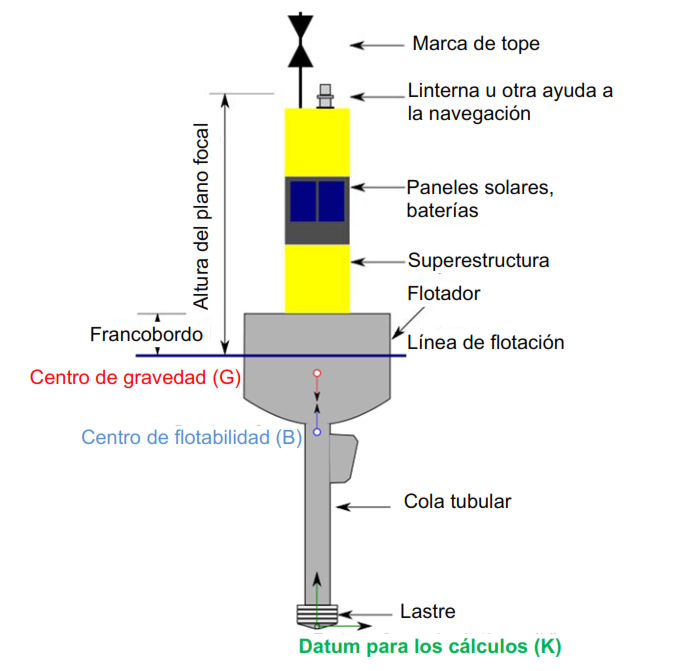
\includegraphics[width=0.7\textwidth]{Documento/Imagenes/Marco Teorico/boya_centro.png}
\caption{Relación entre centro de gravedad (G), centro de flotación (B) y metacentro (M). Fuente: Guía IALA G1099 \cite{IALA_2013_Hydrostatic}.}
\label{fig:metacentrica}
\end{figure}

\begin{figure}[H]
\centering
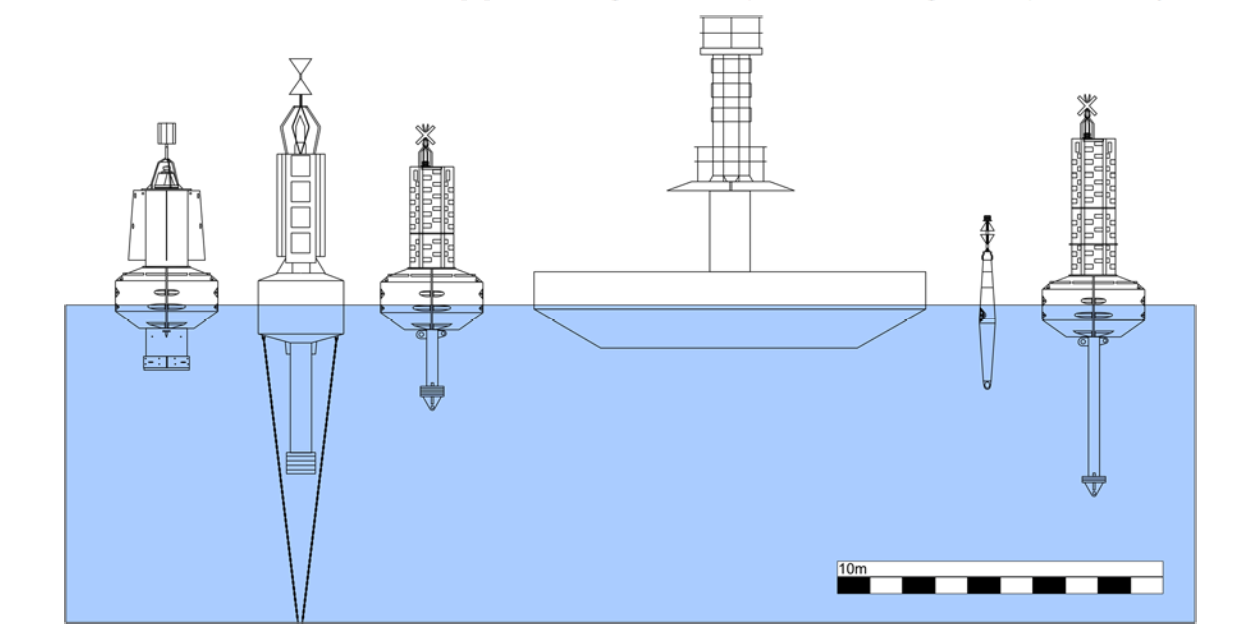
\includegraphics[width=0.85\textwidth]{Documento/Imagenes/Marco Teorico/tipos_boyas.png}
\caption{Formas geométricas típicas de boyas fluviales. Fuente: Guía IALA G1099.}
\label{fig:formas_boyas}
\end{figure}

\end{comment}